\section{MÔ PHỎNG VÀ KIỂM THỬ HỆ THỐNG NIOS V VÀ DMA}
\label{sec:chapter4_content} % Changed label from Chapter4
Mô phỏng (Simulation) là một bước quan trọng trong quy trình thiết kế \acrshort{fpga}, cho phép xác minh chức năng của thiết kế phần cứng và sự tương tác giữa các thành phần trước khi triển khai lên phần cứng vật lý. Việc này giúp phát hiện lỗi sớm, tiết kiệm thời gian và công sức gỡ lỗi trên bo mạch thực tế. Chương này trình bày quy trình mô phỏng, công cụ sử dụng, và kết quả kiểm thử chức năng của bộ điều khiển \acrshort{dma} tùy chỉnh được tích hợp trong hệ thống \acrshort{soc} \acrlong{niosv}.
\subsection{Công cụ Mô phỏng và Yêu cầu Môi trường}

Công cụ chính được sử dụng để mô phỏng hệ thống trong dự án này là \textbf{Questa Advanced Simulator} (trước đây là ModelSim-Intel FPGA Edition), một trình mô phỏng HDL mạnh mẽ được cung cấp bởi Siemens.

Khác với \acrshort{nios2}, hệ thống \acrshort{niosv} không hỗ trợ Generate Testbench System với các phiên bản Quartus Prime Lite và Standard trên hệ điều hành Windows (và Intel cũng đã thông báo sẽ không hỗ trợ cho việc này trên hệ điều hành Windows \cite{intel-forum-simulation}). Do đó, có hai phương pháp chính để tạo testbench mô phỏng cho hệ thống \acrshort{niosv}:

\begin{enumerate}
    \item \textbf{Sử dụng Quartus Prime Pro:} Phiên bản Pro hỗ trợ đầy đủ việc tạo testbench cho \acrshort{niosv} trên Windows, tuy nhiên phiên bản này yêu cầu giấy phép (license) khác, và tốn dung lượng ổ cứng từ 40-145 GB.
    \item \textbf{Generate Testbench System trên Linux:} Thực hiện cài đặt Quartus Prime (Lite hoặc Standard) trên một môi trường Linux. Sử dụng Platform Designer trên Linux để "Generate Testbench System" cho tệp \texttt{system.qsys}. Sau khi testbench được tạo thành công trên Linux (như minh họa trong Hình \ref{fig:04_01_UbuntuGenerateTestbenchSystem}), toàn bộ thư mục project (bao gồm cả thư mục testbench đã tạo) có thể được sao chép sang môi trường Windows để thực hiện các bước mô phỏng tiếp theo bằng QuestaSim trên Windows. Quy trình chi tiết cho việc này được mô tả trong Phụ lục \ref{sec:generate_tb_system}.
\end{enumerate}

\begin{figure}[htbp]
    \centering
    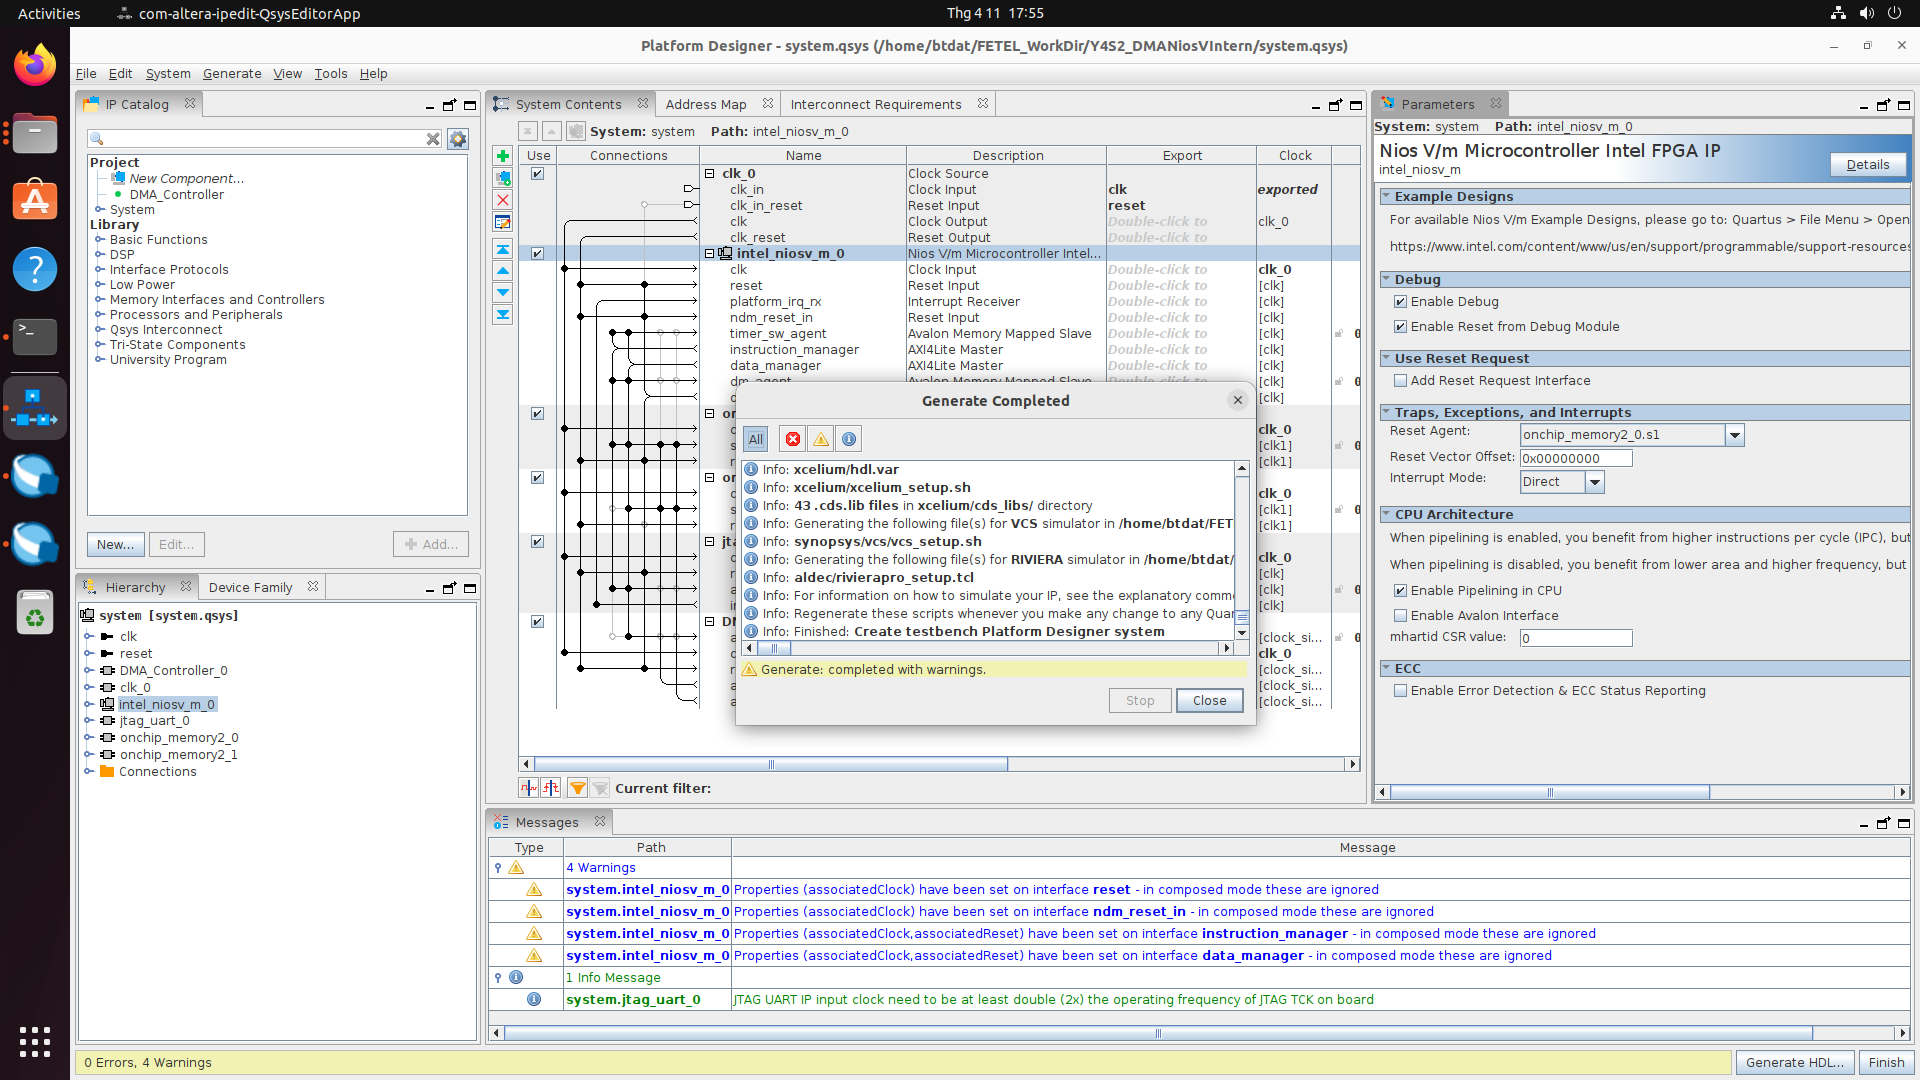
\includegraphics[width=\linewidth]{Images/04_00_UbuntuGenerateTestbenchSystem.png}
    \caption{Generate Testbench System trong Platform Designer trên Ubuntu 22.04.5 thành công.}
    \label{fig:04_01_UbuntuGenerateTestbenchSystem}
\end{figure}

Ngoài ra, để mô phỏng hoạt động của bộ xử lý \acrshort{niosv} thực thi mã phần mềm kiểm thử \acrshort{dma}, tệp chương trình thực thi (\texttt{.elf}) cần được biên dịch (như mô tả ở Phần \ref{sec:chapter3_content}) và sau đó chuyển đổi thành định dạng bộ nhớ (\texttt{.hex}) \cite{intelNiosVSoftwareDevHandbook}. Các tệp \texttt{.hex} này sẽ được testbench tự động nạp vào mô hình bộ nhớ \acrshort{ram} on-chip trong quá trình khởi tạo mô phỏng, cho phép bộ xử lý \acrshort{niosv} mô phỏng thực thi chương trình và tương tác với bộ điều khiển \acrshort{dma} \cite{intelNiosVHandbook}.

\subsection{Kết quả mô phỏng và kiểm thử chức năng}
\label{sec:simulation_results} % Added label

Mục tiêu của mô phỏng là xác minh rằng bộ điều khiển \acrshort{dma} tùy chỉnh hoạt động đúng theo thiết kế: nhận cấu hình từ \acrshort{niosv}, thực hiện truyền dữ liệu giữa hai vùng nhớ on-chip một cách độc lập, và báo hiệu hoàn thành chính xác. Mô phỏng được thực hiện bằng Questa Sim \cite{intelNiosVHandbook}, sử dụng testbench được tạo ra theo quy trình ở Mục \ref{sec:generate_tb_system} và Phụ lục \ref{sec:generate_tb_system}.

Quá trình mô phỏng bao gồm các bước chính sau, được minh họa bằng các dạng sóng tín hiệu Avalon-MM Slave và Master của bộ điều khiển \acrshort{dma}:

\begin{enumerate}
    \item \textbf{Cấu hình DMA qua giao diện Slave:} Bộ xử lý \acrshort{niosv} (được mô phỏng thực thi mã trong tệp \texttt{.hex}) ghi các thông số cần thiết vào các thanh ghi của module \texttt{CONTROL\_SLAVE} thông qua giao diện Avalon-MM Slave.
    \begin{itemize}
        \item Ghi địa chỉ bắt đầu đọc (Source Address) vào thanh ghi tại offset 0 (Hình \ref{fig:04_01_ControlSlave_Write_RM_startaddress}).
        \item Ghi địa chỉ bắt đầu ghi (Destination Address) vào thanh ghi tại offset 1 (Hình \ref{fig:04_02_ControlSlave_Write_WM_startaddress}).
        \item Ghi độ dài dữ liệu cần truyền (tính bằng byte) vào thanh ghi tại offset 2 (Hình \ref{fig:04_03_ControlSlave_Write_Length}).
    \end{itemize}

    \item \textbf{Khởi động DMA Transfer:} Sau khi cấu hình xong, \acrshort{niosv} ghi giá trị 1 vào bit 0 (bit GO) của thanh ghi điều khiển (Control Register) tại offset 4. Thao tác ghi này (tín hiệu \texttt{iWrite=1}, \texttt{iAddress=4}, \texttt{iWritedata[0]=1}) được \texttt{CONTROL\_SLAVE} phát hiện, và nó sẽ kích hoạt tín hiệu \texttt{Start} nội bộ, báo hiệu cho các module Master bắt đầu hoạt động (Hình \ref{fig:04_04_DMA_Start_control_go}).

    \item \textbf{Quá trình truyền dữ liệu (Read Master và Write Master):}
    \begin{itemize}
        \item Module \texttt{READ\_MASTER} bắt đầu tạo các giao dịch đọc Avalon-MM từ địa chỉ nguồn đã cấu hình, đọc dữ liệu và đẩy vào FIFO.
        \item Khi FIFO có dữ liệu (\texttt{FF\_empty=0}), module \texttt{WRITE\_MASTER} bắt đầu đọc dữ liệu từ FIFO và tạo các giao dịch ghi Avalon-MM đến địa chỉ đích đã cấu hình.
        \item Quá trình đọc và ghi này diễn ra song song (pipelined) cho đến khi đủ số byte yêu cầu đã được truyền. Hình \ref{fig:04_05_RM_Done} minh họa thời điểm module \texttt{READ\_MASTER} hoàn thành việc đọc toàn bộ dữ liệu từ nguồn và ghi vào FIFO.
    \end{itemize}

    \item \textbf{Hoàn thành DMA Transfer:} Sau khi \texttt{WRITE\_MASTER} ghi xong word dữ liệu cuối cùng vào bộ nhớ đích, nó sẽ kích hoạt tín hiệu \texttt{WM\_done=1}. Module \texttt{CONTROL\_SLAVE} nhận tín hiệu này, cập nhật thanh ghi trạng thái (Status Register) bằng cách đặt bit DONE (\texttt{status\_done=1}) và xóa bit BUSY (\texttt{status\_busy=0}), đồng thời tự động xóa bit GO (\texttt{control\_go=0}) để kết thúc phiên truyền (Hình \ref{fig:04_06_DMA_Done}). Bộ xử lý \acrshort{niosv} có thể đọc thanh ghi trạng thái để biết khi nào quá trình \acrshort{dma} hoàn tất.

    \item \textbf{Kết quả tổng thể:} Cửa sổ Transcript của Questa Sim (Hình \ref{fig:04_07_TranscriptSimulationOutput}) ghi lại log của quá trình mô phỏng, bao gồm các thông báo từ testbench hoặc mã phần mềm \acrshort{niosv} (nếu có \texttt{printf}), xác nhận các bước thực hiện và kết quả cuối cùng của việc truyền dữ liệu.
\end{enumerate}

% Figures illustrating the simulation steps
\begin{figure}[htbp]
    \centering
    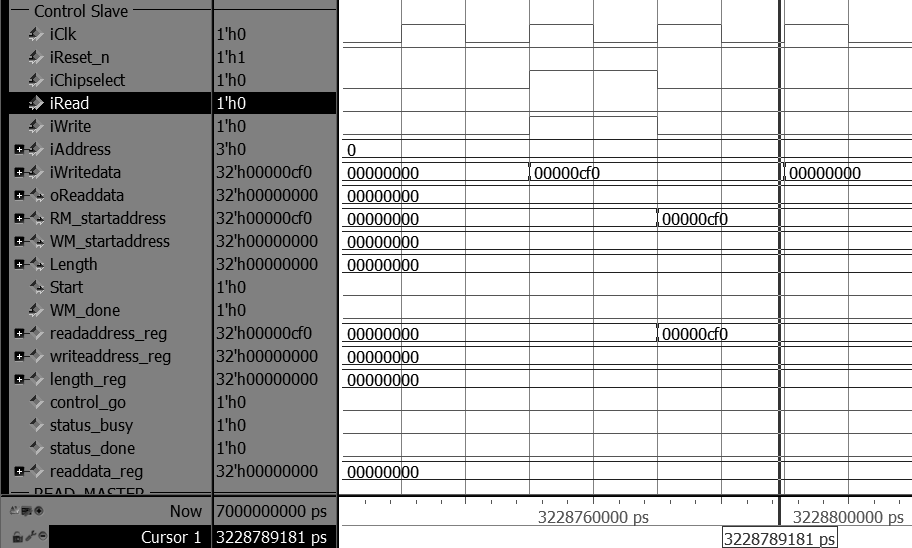
\includegraphics[width=0.7\linewidth]{Images/04_01_ControlSlave_Write_RM_startaddress.png} % Reduced width slightly
    \caption{Mô phỏng: Ghi địa chỉ Read Master Start Address vào giao diện DMA Control Slave.}
    \label{fig:04_01_ControlSlave_Write_RM_startaddress}
\end{figure}

\begin{figure}[htbp]
    \centering
    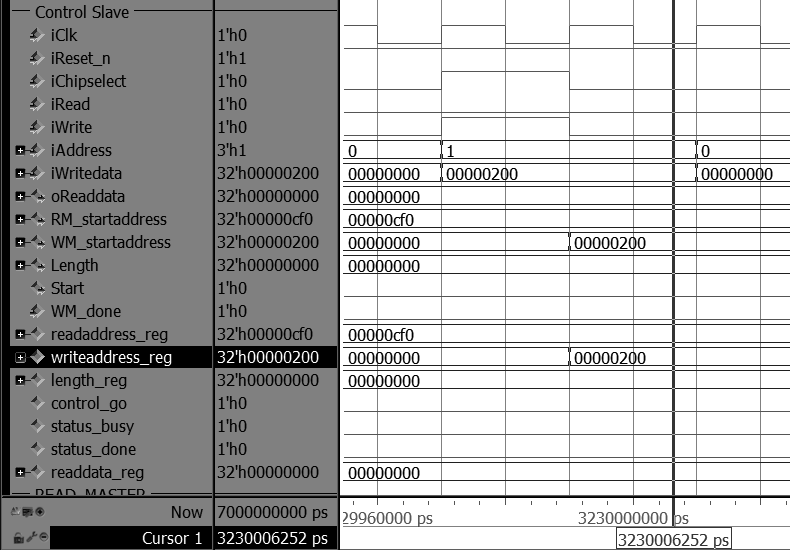
\includegraphics[width=0.8\linewidth]{Images/04_02_ControlSlave_Write_WM_startaddress.png} % Reduced width slightly
    \caption{Mô phỏng: Ghi địa chỉ Write Master Start Address vào giao diện DMA Control Slave.}
    \label{fig:04_02_ControlSlave_Write_WM_startaddress}
\end{figure}

\begin{figure}[htbp]
    \centering
    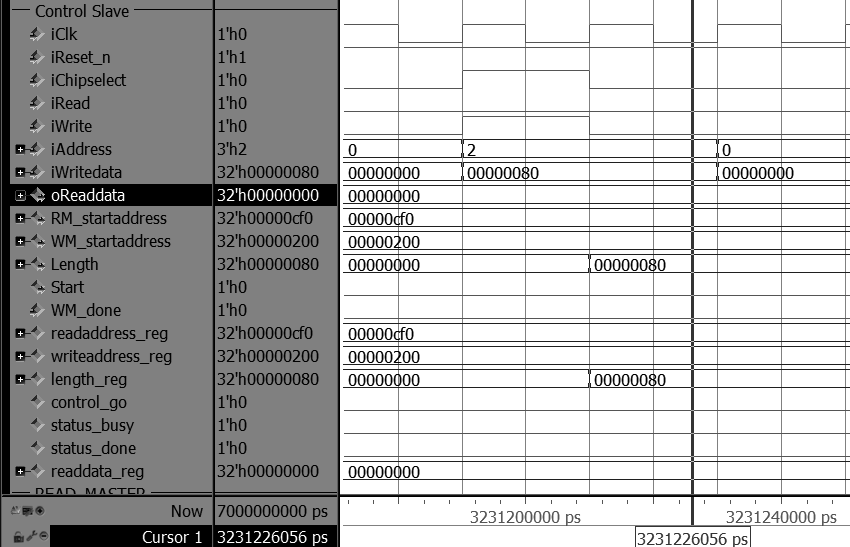
\includegraphics[width=0.8\linewidth]{Images/04_03_ControlSlave_Write_Length.png} % Reduced width slightly
    \caption{Mô phỏng: Thiết lập độ dài truyền (Transfer Length) qua giao diện DMA Control Slave.}
    \label{fig:04_03_ControlSlave_Write_Length}
\end{figure}

\begin{figure}[htbp]
    \centering
    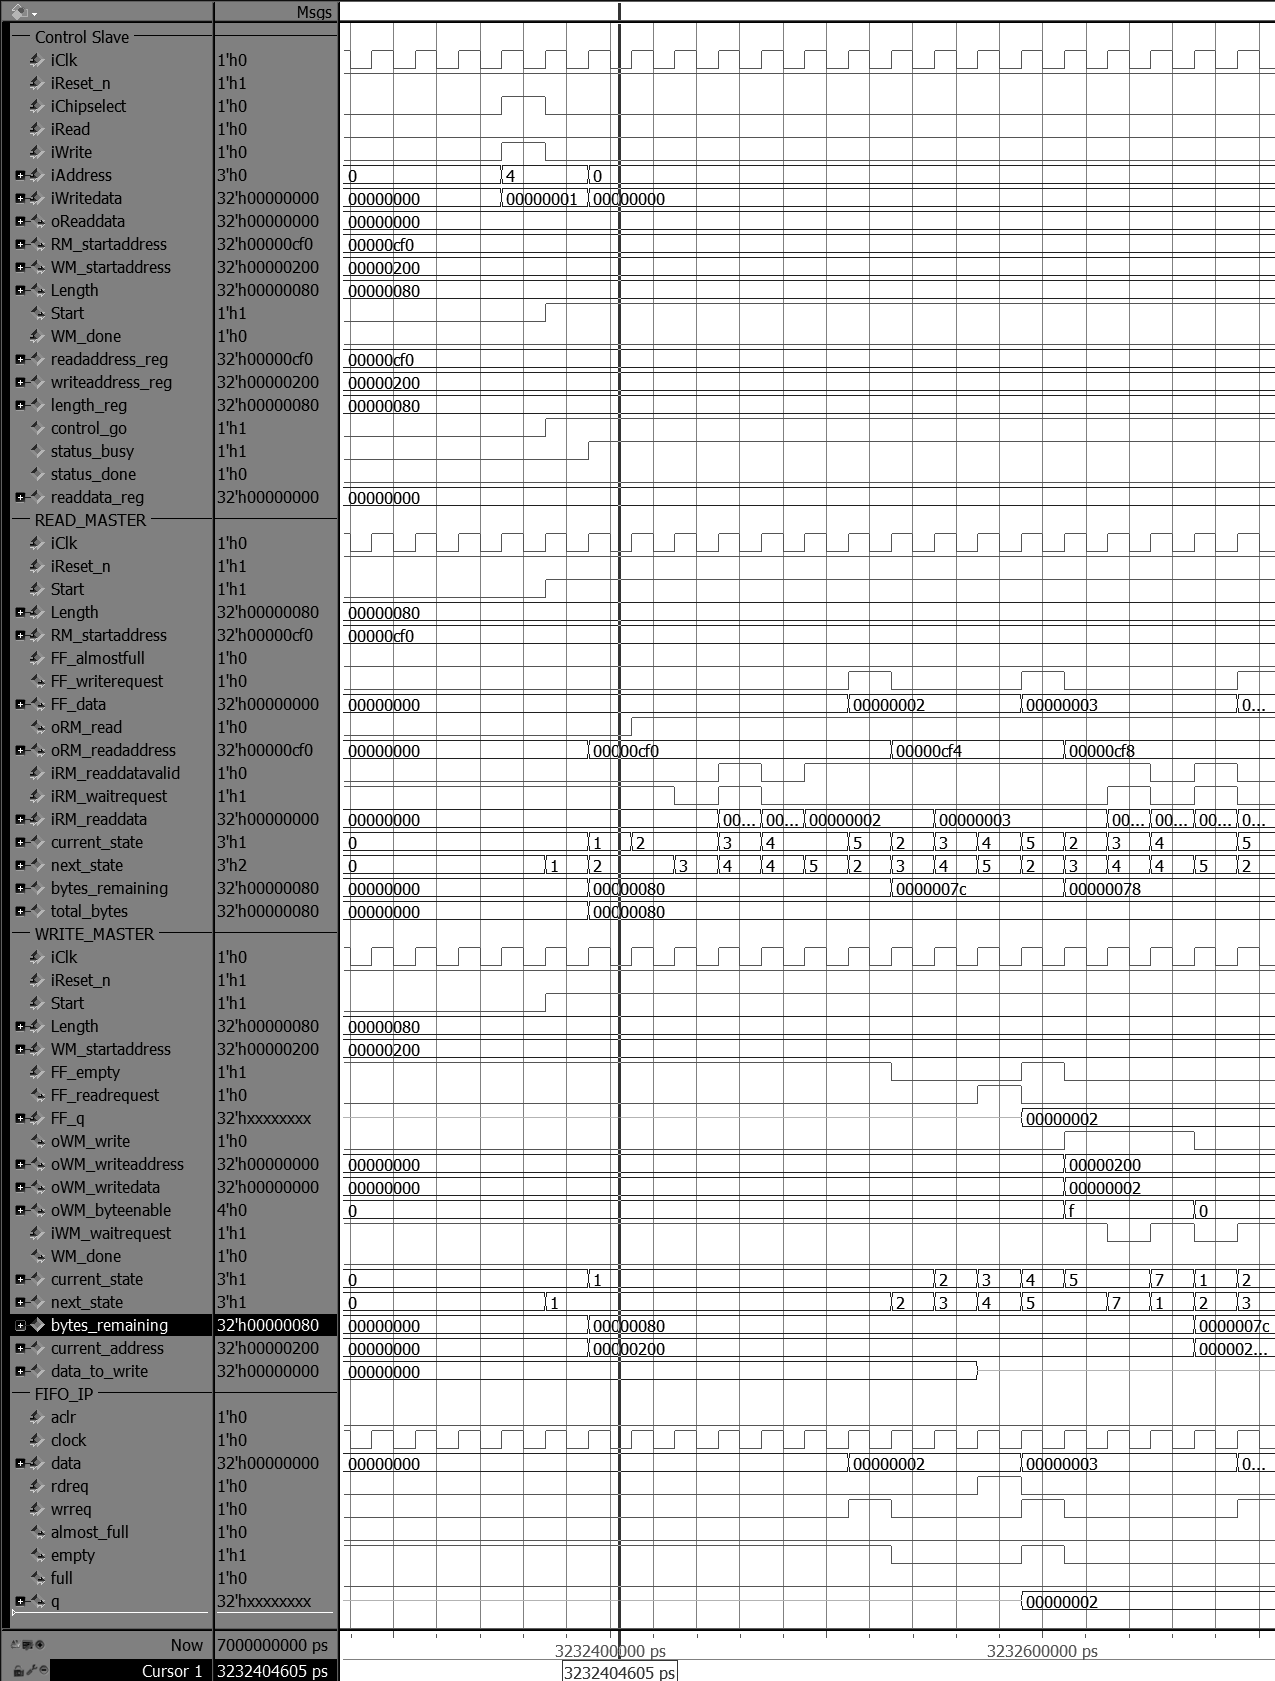
\includegraphics[width=\linewidth]{Images/04_04_DMA_Start_control_go.png}
    \caption{Mô phỏng: Khởi tạo truyền DMA bằng cách đặt bit Control GO.}
    \label{fig:04_04_DMA_Start_control_go}
\end{figure}

\begin{figure}[htbp]
    \centering
    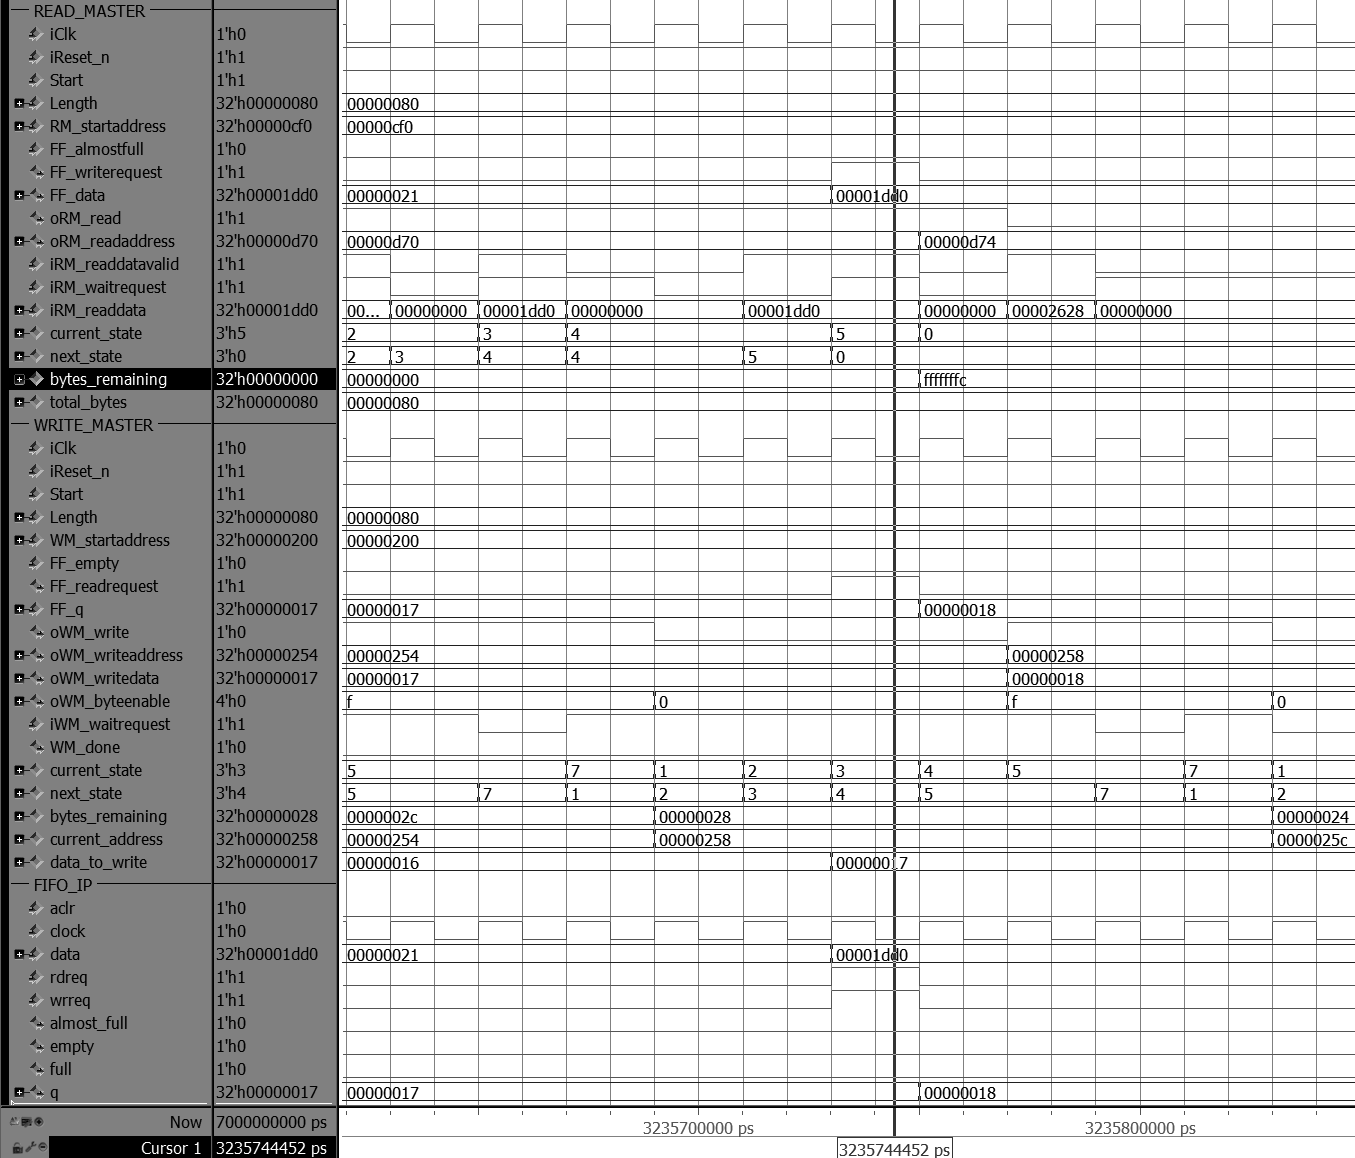
\includegraphics[width=\linewidth]{Images/04_05_RM_Done.png}
    \caption{Mô phỏng: Hoàn thành các hoạt động của Read Master trong quá trình truyền DMA.}
    \label{fig:04_05_RM_Done}
\end{figure}

\begin{figure}[htbp]
    \centering
    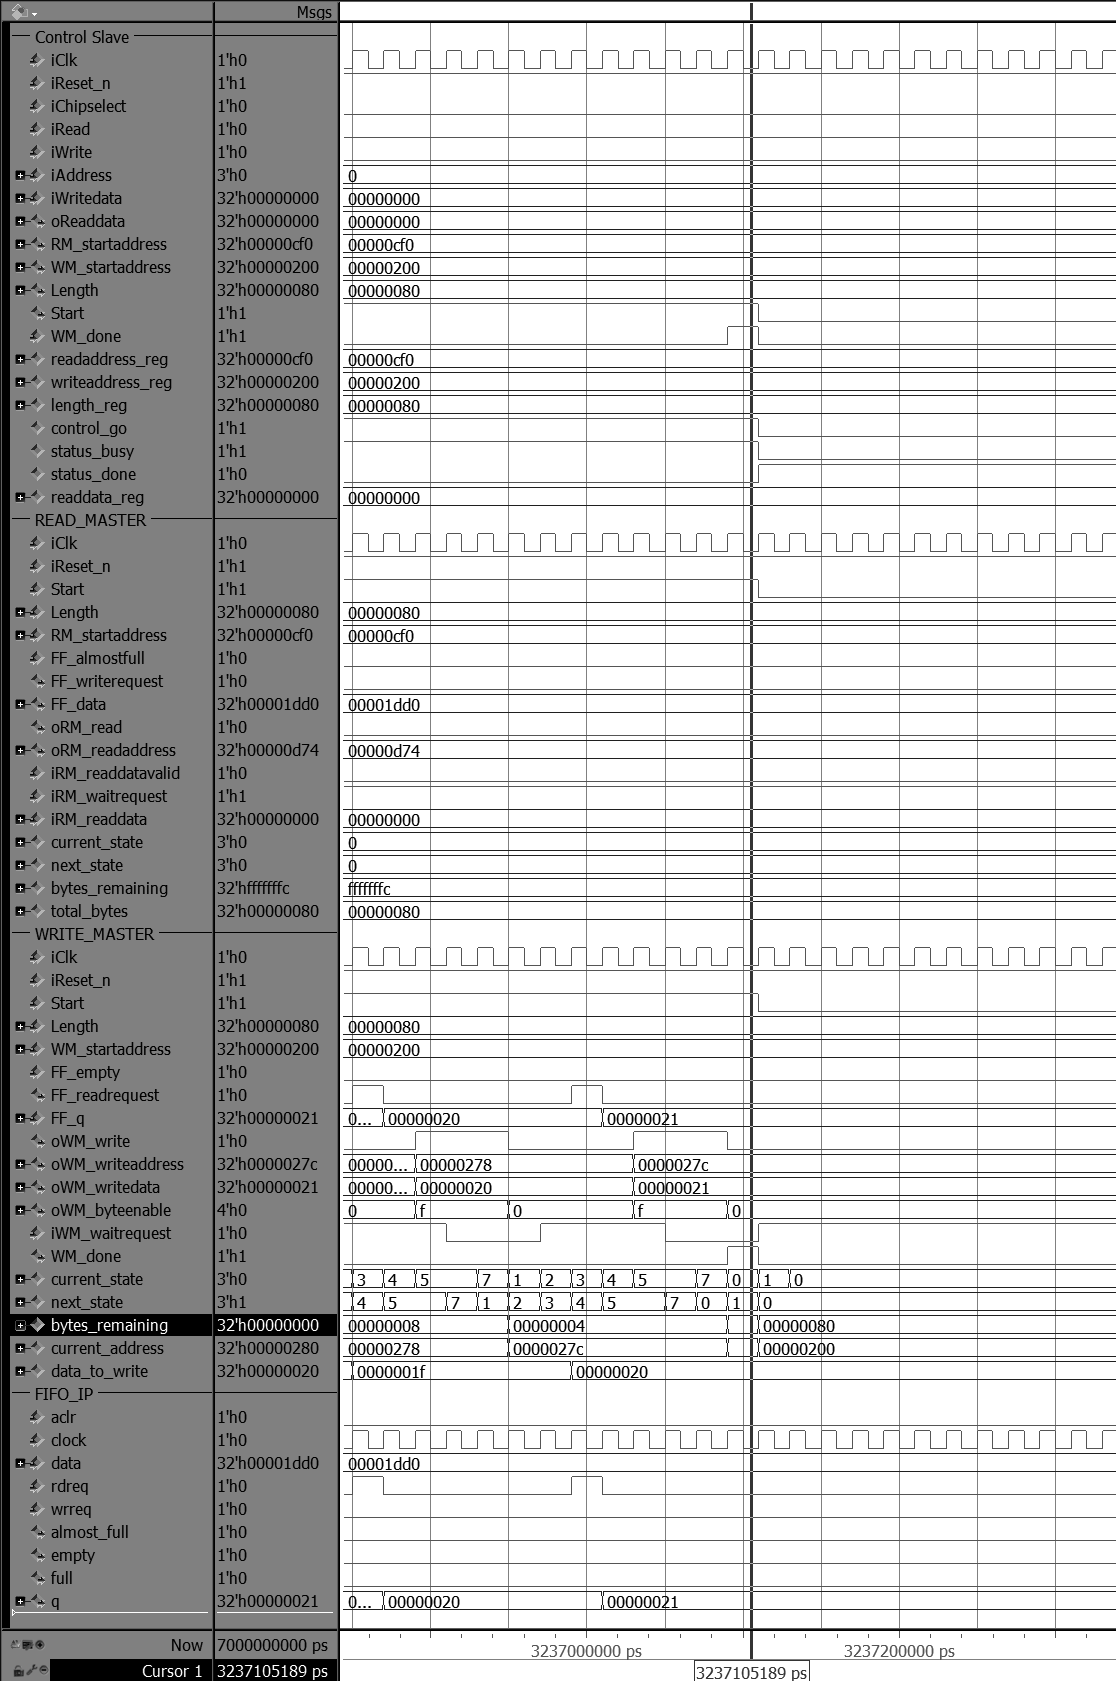
\includegraphics[width=0.8\linewidth]{Images/04_06_DMA_Done.png}
    \caption{Mô phỏng: Tín hiệu hoàn thành (WM\_done và status\_done) cho biết truyền DMA thành công.}
    \label{fig:04_06_DMA_Done}
\end{figure}

\begin{figure}[htbp]
    \centering
    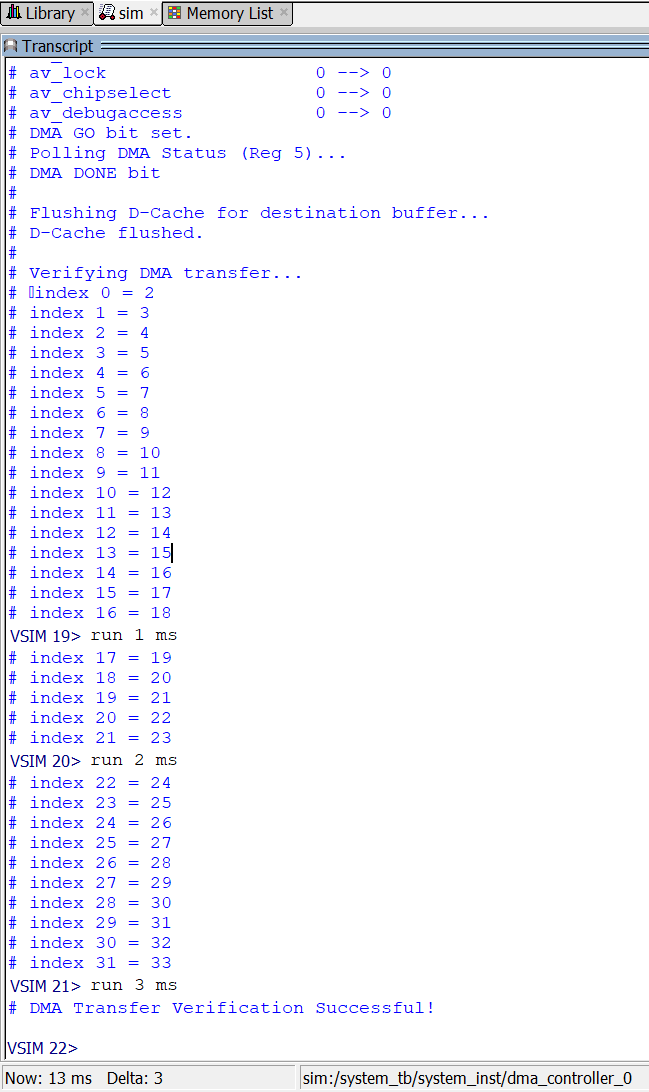
\includegraphics[width=0.7\linewidth]{Images/04_07_TranscriptSimulationOutput.png} % Adjusted width
    \caption{Mô phỏng: Transcript hiển thị quá trình và kết quả truyền DMA.}
    \label{fig:04_07_TranscriptSimulationOutput}
\end{figure}

\FloatBarrier % Ensure all figures are placed before the conclusion

\subsection{Kết luận Phần Mô phỏng} % Renamed section
\label{sec:chapter4_conclusion} % Kept label, but section name changed

Quá trình mô phỏng hệ thống \acrshort{soc} \acrshort{niosv} tích hợp bộ điều khiển \acrshort{dma} tùy chỉnh đã được thực hiện thành công bằng công cụ Questa Advanced Simulator. Các kết quả mô phỏng, được thể hiện qua các dạng sóng tín hiệu Avalon và cửa sổ transcript (Hình \ref{fig:04_01_ControlSlave_Write_RM_startaddress} đến \ref{fig:04_07_TranscriptSimulationOutput}), đã xác minh các chức năng chính của bộ điều khiển \acrshort{dma}:
\begin{itemize}
    \item Khả năng nhận cấu hình (địa chỉ nguồn, đích, độ dài) từ bộ xử lý \acrshort{niosv} thông qua giao diện Avalon-MM Slave.
    \item Khả năng khởi động quá trình truyền dữ liệu khi nhận được lệnh GO.
    \item Hoạt động độc lập của các module Read Master và Write Master trong việc đọc dữ liệu từ nguồn, đệm qua FIFO, và ghi dữ liệu vào đích, tuân thủ đúng giao thức Avalon-MM \cite{avalon_mm_transfer}.
    \item Khả năng báo hiệu hoàn thành (DONE) một cách chính xác sau khi hoàn tất việc truyền dữ liệu.
\end{itemize}
Kết quả mô phỏng khẳng định thiết kế bộ điều khiển \acrshort{dma} hoạt động đúng như mong đợi ở cấp độ \acrfull{rtl}, tạo tiền đề vững chắc cho việc triển khai và kiểm thử trên phần cứng \acrshort{fpga} thực tế được trình bày ở Phần \ref{sec:chapter3_content}. % Updated reference

\FloatBarrier % Ensure conclusion text appears at the end